\documentclass[11pt]{article}

% --- Packages (all standard on Overleaf) ---
\usepackage[T1]{fontenc}
\usepackage[utf8]{inputenc}
\usepackage[a4paper,margin=22mm]{geometry}
\usepackage{amsmath}
\usepackage{booktabs}
\usepackage{graphicx}
\usepackage{xcolor}
\usepackage{tikz}
\usetikzlibrary{arrows.meta,positioning,fit,backgrounds}
\usepackage[hidelinks]{hyperref}
\usepackage{caption}
\captionsetup{font=small,labelfont=bf}

% --- Light styling ---
\definecolor{ink}{HTML}{1b3a6b}
\newcommand{\code}[1]{\texttt{\small #1}}

\title{\vspace{-6mm}\textbf{The SignCollect Annotation Tool v3:\\
Automatic Sign Segmentation and Gloss Spotting in the Browser}}
\author{G.\ Otterspeer\\[2pt]
\small SignCollect $\cdot$ Global Signbank, University of Amsterdam\\
\small Technical Report $\cdot$ June 2026 $\cdot$ \code{signcollect.nl/annotation-tool}}
\date{}

% --- TikZ shared styles ---
\tikzset{
  box/.style={draw=ink, rounded corners=3pt, align=center, inner sep=4pt, font=\small},
  fbox/.style={box, fill=ink!6},
  wbox/.style={box, fill=white},
  flow/.style={-{Latex[length=2mm]}, draw=ink, thick},
  lbl/.style={font=\scriptsize\itshape, text=black!60},
}

\begin{document}
\maketitle
\thispagestyle{empty}

\begin{abstract}
\noindent We describe version~3 of the SignCollect annotation tool, a browser-based editor for
multi-tier annotation of sign-language video that now closes the loop between \emph{recording}
and \emph{annotation} by embedding two neural models directly into the editing workflow. When a
user drops a clip into the tool, a \emph{sign segmentation} model based on a frozen V-JEPA~2
video backbone and a recurrent (BiLSTM) frame-labelling head partitions the continuous signing
stream into individual sign segments; each resulting segment is then passed to a
\emph{sign-spotting} model that encodes the clip with a self-supervised sign representation
(SignRep, built on a Hiera vision transformer) and matches it against a 10{,}254-gloss
dictionary, returning a ranked list of candidate glosses. Both models run as warm GPU inference
services reached over HTTPS, so the entire segment-then-gloss pipeline executes in seconds
without the annotator leaving the page. On the Zin-in-NGT benchmark the deployed segmenter
attains a boundary F1 of $0.871$ using RGB alone (no pose extraction), via a
BiLSTM~$\times$~MS-TCN probability ensemble; the single BiLSTM head reaches $0.817$--$0.848$
depending on frame rate. We detail the model architectures, the system design that makes them
usable from a single-page application, and the resulting human-in-the-loop annotation workflow.

\smallskip
\noindent\textbf{Keywords:} sign language, NGT, annotation tooling, temporal segmentation, sign
spotting, self-supervised video representation, Global Signbank.
\end{abstract}

\section{Introduction}
Constructing large sign-language repositories is bottlenecked less by recording than by
annotation: raw video must be cut into individual signs and each sign must be labelled with a
gloss linked to a lexical database. The SignCollect pipeline~\cite{signcollect} addressed the
capture side with a touchless, multi-view recording setup that lets the Sign Language of the
Netherlands (NGT) lexicon in Global Signbank be extended quickly. The annotation tool described
here addresses the downstream side, and version~3 (v3) adds machine assistance to the two most
repetitive manual steps---temporal segmentation and gloss assignment.

The tool remains a single self-contained web application: a multi-tier timeline editor that
loads a video (and optionally an existing ELAN \code{.eaf} file), lets an annotator create, move
and label segments, and exports the result as EAF. v3 keeps this editor unchanged but augments
it so that, on dropping a fresh clip, the timeline is pre-populated with predicted sign
boundaries and each predicted segment is pre-annotated with the ten most likely glosses. The
annotator's task shifts from authoring from scratch to verifying and correcting---a
substantially faster mode of work.

This report concentrates on the two models and the engineering that makes them usable from the
browser. Section~\ref{sec:system} gives the system architecture. Sections~\ref{sec:seg}
and~\ref{sec:spot} describe the segmentation and spotting models. Section~\ref{sec:deploy}
describes the human-in-the-loop workflow and deployment, Section~\ref{sec:results} reports
benchmark results, and Section~\ref{sec:disc} discusses limitations.

\section{System overview}\label{sec:system}
The browser application normalises every dropped video to 25 frames per second and H.264 at
$\leq$1080p (using an in-page WebAssembly build of FFmpeg) so that the models always receive a
fixed frame rate. It then issues two kinds of HTTPS requests: a single \code{/segment} call
carrying the whole clip, and one \code{/spot} call per detected segment. Neither model runs in
the browser; each is a \emph{warm} inference service---a long-lived process that loads its model
weights once and keeps them resident on the GPU---so per-request latency is dominated by
computation, not model loading.

Because the GPU host is not publicly reachable, the public web server exposes the two services
through Apache reverse-proxy paths (\code{/sign-spotter/} and \code{/sign-segmenter/}) that
forward to local ports (8000 and 8001) bridged to the GPU host by persistent SSH tunnels
(Figure~\ref{fig:arch}). Warm, this yields roughly 1~s per gloss-spotting call (a four-sign clip
on an RTX~6000~Ada) and several seconds for whole-clip segmentation.

\begin{figure}[t]
\centering
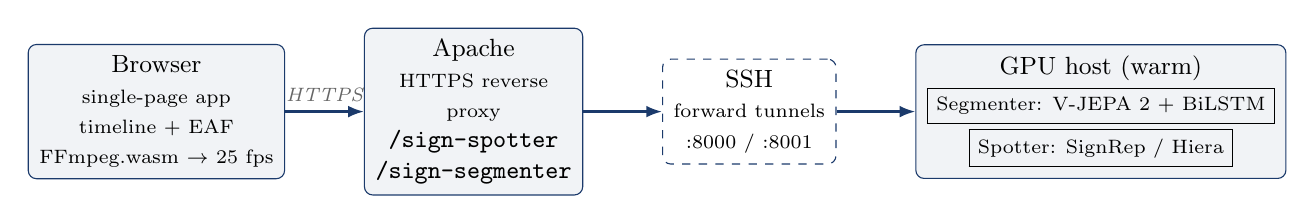
\begin{tikzpicture}[node distance=10mm]
\node[fbox] (browser) {Browser\\\scriptsize single-page app\\\scriptsize timeline + EAF\\\scriptsize FFmpeg.wasm $\to$ 25 fps};
\node[fbox, right=of browser] (apache) {Apache\\\scriptsize HTTPS reverse\\\scriptsize proxy\\\scriptsize \code{/sign-spotter}\\\scriptsize \code{/sign-segmenter}};
\node[wbox, right=of apache, draw=ink, dashed] (ssh) {SSH\\\scriptsize forward tunnels\\\scriptsize :8000 / :8001};
\node[fbox, right=of ssh] (gpu) {GPU host (warm)\\[2pt]
  \fbox{\scriptsize Segmenter: V-JEPA 2 + BiLSTM}\\[1pt]
  \fbox{\scriptsize Spotter: SignRep / Hiera}};
\draw[flow] (browser) -- node[lbl,above]{HTTPS} (apache);
\draw[flow] (apache) -- (ssh);
\draw[flow] (ssh) -- (gpu);
\end{tikzpicture}
\caption{System architecture. The browser performs all editing locally and calls two stateless
HTTPS endpoints. An Apache reverse proxy forwards them across persistent SSH tunnels to warm
inference services on a multi-GPU host, which keep both models resident to minimise latency.}
\label{fig:arch}
\end{figure}

\section{Sign segmentation model}\label{sec:seg}
The segmenter answers a single question for every frame: is the signer mid-sign, and where do
signs begin and end? It is deliberately \emph{RGB-only}---it needs no hand- or body-pose
extraction---which removes a brittle and expensive preprocessing stage. The model has two parts:
a large \emph{frozen} video backbone that turns frames into rich features, and a small trained
head that reads those features as a time series and emits boundaries (Figure~\ref{fig:seg}).

\subsection{Frozen V-JEPA 2 backbone}
Features come from V-JEPA~2~\cite{vjepa2}, a ViT-L video encoder
(\code{vjepa2-vitl-fpc64-256}) pre-trained self-supervisedly on over a million hours of general
internet video---not on sign language. V-JEPA~2 is a Joint-Embedding Predictive Architecture:
rather than reconstructing pixels, it learns to predict the latent features of masked
spatiotemporal regions, yielding representations that capture motion and scene dynamics. We use
it strictly as a frozen feature extractor.

The encoder is run on non-overlapping 16-frame chunks. Each forward pass produces a temporal
grid of patch tokens which we pool into a $3\times3$ spatial grid, giving nine region tokens
(one per region) of dimension 1024 for each of eight temporal positions in the chunk. To raise
the effective temporal resolution to one token per frame, we use a \emph{phase-dual} scheme: the
backbone is run twice per chunk, once on the frames as-is and once on the same frames shifted by
one, and the two phase-shifted token streams are interleaved. The result is a sequence of one
$9\times1024$ region-token vector per frame at 25~Hz.

\subsection{Region BiLSTM head and BIO decoding}
The trained head (\code{RegionBiLSTM}) first collapses the nine region tokens at each frame into
a single vector using a small \emph{learned-query attention pool}, so the model can weight, say,
the dominant-hand region. The pooled per-frame sequence is then processed by a bidirectional
LSTM, which reads the whole clip in both directions so each frame is labelled in the context of
its neighbours. A temporal smoothing (T-MSE) loss discourages jittery frame-to-frame label
flips. The deployed default further \emph{ensembles} this BiLSTM with a sibling three-stage
dilated-residual temporal convolutional head in the style of MS-TCN~\cite{mstcn}, averaging
their per-frame label probabilities; the ensemble is what the served model uses, while either
head can run alone.

The head emits, per token, one of three \emph{BIO} labels---\code{OUT} (no sign), \code{IN}
(inside a sign), \code{BEGIN} (first frame of a sign). The token labels are upsampled to the
25~fps frame grid, lightly cleaned, and every maximal run of non-\code{OUT} frames is emitted as
one \code{(start, end)} segment in seconds. These segments become the timeline boxes the
annotator sees. The head was pre-trained on the German MeineDGS corpus and then fine-tuned on
Zin-in-NGT, selecting the checkpoint with the best validation boundary F1.

\begin{figure}[t]
\centering
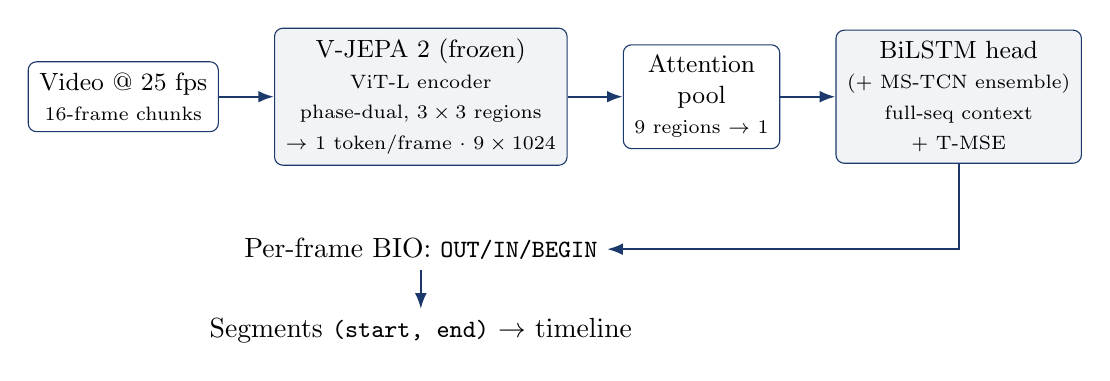
\begin{tikzpicture}[node distance=7mm]
\node[wbox] (v) {Video @ 25 fps\\\scriptsize 16-frame chunks};
\node[fbox, right=of v] (b) {V-JEPA 2 (frozen)\\\scriptsize ViT-L encoder\\\scriptsize phase-dual, $3\times3$ regions\\\scriptsize $\to$ 1 token/frame $\cdot$ $9\times1024$};
\node[wbox, right=of b] (p) {Attention\\pool\\\scriptsize 9 regions $\to$ 1};
\node[fbox, right=of p] (h) {BiLSTM head\\\scriptsize (+ MS-TCN ensemble)\\\scriptsize full-seq context\\\scriptsize + T-MSE};
\node[below=8mm of b] (bio) {Per-frame BIO: \code{OUT/IN/BEGIN}};
\node[below=5mm of bio] (seg) {Segments \code{(start, end)} $\to$ timeline};
\draw[flow] (v) -- (b);
\draw[flow] (b) -- (p);
\draw[flow] (p) -- (h);
\draw[flow] (h.south) |- (bio.east);
\draw[flow] (bio) -- (seg);
\end{tikzpicture}
\caption{Segmentation pipeline. A frozen V-JEPA~2 backbone turns 25~fps frames into one
$9\times1024$ region-token vector per frame; an attention pool plus a BiLSTM head (ensembled
with an MS-TCN sibling at serve time) labels each frame \code{OUT/IN/BEGIN}; contiguous
non-\code{OUT} runs become timeline segments.}
\label{fig:seg}
\end{figure}

\section{Sign-spotting model}\label{sec:spot}
Given a segment, the spotter proposes which lexical sign it is. It treats spotting as
\emph{nearest-neighbour retrieval in an embedding space}~\cite{momeni} rather than as
fixed-class classification, which lets the vocabulary grow simply by adding dictionary
entries---no retraining required.

\subsection{SignRep encoder}
The segment clip is encoded by SignRep~\cite{signrep}, a self-supervised sign representation
built on a Hiera hierarchical vision transformer~\cite{hiera}. SignRep is trained as a masked
autoencoder that injects sign-specific inductive priors (skeleton-based cues) during
pre-training but, crucially, requires \emph{no} keypoints at inference time; it also uses
feature regularisation and a style-agnostic adversarial loss to make the embedding robust to
signer appearance. The encoder maps a variable-length clip to a single 768-dimensional embedding
vector.

The base SignRep encoder is adapted to NGT by supervised-contrastive fine-tuning. The deployed
spotter is in fact a small \emph{ensemble} of two such fine-tuned backbones (two independent
fine-tuning rounds): each segment is embedded by both, scored against the dictionary, and the
two score lists are combined by per-segment z-normalised fusion. This ensemble is the default
served configuration; a single backbone can be used as a lighter fallback.

\subsection{Dictionary matching}
Each gloss in the reference lexicon is represented by a pre-computed embedding. At query time the
segment embedding is compared by cosine similarity against the full dictionary, and the ten
highest-scoring glosses are returned with their scores (Figure~\ref{fig:spot}). The deployed
dictionary is the full-coverage set of \textbf{10{,}254 glosses}, built from the Zin-in-NGT
ground-truth signs together with the Global Signbank studio clips, so the spotter can in
principle propose any sign in that lexicon. In the editor these ten candidates appear in a
dropdown beneath the segment; clicking one fills the segment's gloss field, and hovering a
candidate previews its reference video.

\begin{figure}[t]
\centering
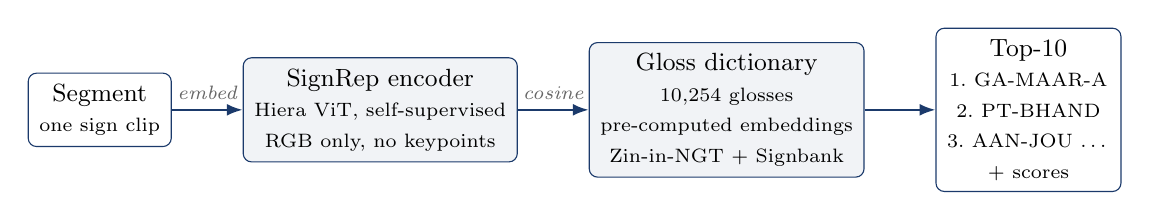
\begin{tikzpicture}[node distance=9mm]
\node[wbox] (s) {Segment\\\scriptsize one sign clip};
\node[fbox, right=of s] (e) {SignRep encoder\\\scriptsize Hiera ViT, self-supervised\\\scriptsize RGB only, no keypoints};
\node[fbox, right=of e] (d) {Gloss dictionary\\\scriptsize 10{,}254 glosses\\\scriptsize pre-computed embeddings\\\scriptsize Zin-in-NGT + Signbank};
\node[wbox, right=of d] (t) {Top-10\\\scriptsize 1.\ GA-MAAR-A\\\scriptsize 2.\ PT-BHAND\\\scriptsize 3.\ AAN-JOU \dots\\\scriptsize + scores};
\draw[flow] (s) -- node[lbl,above]{embed} (e);
\draw[flow] (e) -- node[lbl,above]{cosine} (d);
\draw[flow] (d) -- (t);
\end{tikzpicture}
\caption{Sign-spotting pipeline. A segment clip is encoded by SignRep (a Hiera-based
self-supervised model) into one embedding, which is matched by cosine similarity against
10{,}254 pre-computed gloss embeddings; the ten nearest glosses are returned for the annotator
to choose from.}
\label{fig:spot}
\end{figure}

\section{Annotation workflow and deployment}\label{sec:deploy}
The two models are wired into the editor as a single drop-to-annotate flow:
\begin{enumerate}\itemsep1pt
\item The annotator drops a video; it is normalised to 25 fps in-page.
\item If the clip has no existing segments, the whole video is sent once to \code{/segment}
  while an indeterminate progress bar is shown.
\item Returned segments populate a timeline tier.
\item Each new segment is sent to \code{/spot}; its dropdown first shows a spinner, then the
  top-10 glosses.
\item The annotator confirms or edits boundaries and picks glosses, then exports EAF.
\end{enumerate}
Segmentation runs only when a clip arrives without annotations, so dropping a video alongside an
existing EAF leaves the human's work untouched; a button re-runs segmentation on demand. The
spotter is also invoked whenever the annotator creates a segment by hand, so the assistance is
available throughout editing, not only at import.

Operationally, both services are long-lived HTTP servers that load their model once and keep it
warm. The segmenter is single-process and serialises its GPU calls; the spotter runs a small
pool of replicas---one per GPU---so independent spotting requests can run in parallel across the
host's GPUs. They were deployed on a shared, multi-GPU CUDA host; the public site reaches them
only through the reverse-proxy and SSH-tunnel path of Figure~\ref{fig:arch}. Health endpoints
report which model and dictionary are live so operators can confirm the correct configuration is
serving (the live spotter reports the 10{,}254-gloss coverage dictionary; the live segmenter
reports the BiLSTM~$\times$~MS-TCN ensemble profile).

\section{Results}\label{sec:results}
\subsection{Segmentation}
Table~\ref{tab:seg} reports segmentation quality on the Zin-in-NGT test split (345 sentences),
using RGB alone. The headline metric is \emph{boundary F1}: predicted and reference segment
boundaries (start/end times) are matched greedily one-to-one within a $\pm0.1$~s tolerance, and
F1 is taken over those matches---it measures boundary \emph{timing}, not frame accuracy or
segment count. The deployed model---a BiLSTM~$\times$~MS-TCN probability ensemble---reaches a
boundary F1 of $\mathbf{0.871}$ and a segment F1 of $0.800$. A single BiLSTM head reaches
$0.817$ at 25~fps and $0.848$ at 50~fps (finer frame rate $\Rightarrow$ finer boundary timing);
the MS-TCN head alone is slightly lower ($0.806$). Table~\ref{tab:dgs} summarises cross-lingual
transfer to held-out German (MeineDGS) signing, where performance is lower---as expected for a
model fine-tuned on NGT---but still substantial.

\begin{table}[t]
\centering
\caption{Sign segmentation on Zin-in-NGT (345 sentences), RGB input, boundary tolerance
$\pm0.1$~s. $\pm$4f = within 4 frames. Higher is better.}
\label{tab:seg}
\begin{tabular}{lcccc}
\toprule
V-JEPA~2 head & fps & Bnd F1 & Bnd F1 $\pm$4f & Seg F1 \\
\midrule
\textbf{BiLSTM $\times$ MS-TCN ensemble (deployed)} & 50 & \textbf{0.871} & 0.908 & \textbf{0.800} \\
BiLSTM & 50 & 0.848 & 0.908 & 0.750 \\
BiLSTM & 25 & 0.817 & --- & 0.750 \\
MS-TCN & 25 & 0.806 & 0.903 & 0.739 \\
\bottomrule
\end{tabular}
\end{table}

\begin{table}[t]
\centering
\caption{Cross-lingual transfer to held-out MeineDGS/DGS (boundary / segment F1).}
\label{tab:dgs}
\begin{tabular}{lcc}
\toprule
V-JEPA~2 / Hiera head & Boundary F1 & Segment F1 \\
\midrule
V-JEPA~2 (MS-TCN head) & 0.643 & 0.481 \\
Hiera (MS-TCN head)    & 0.655 & 0.502 \\
\bottomrule
\end{tabular}
\end{table}

\subsection{Spotting}
The spotter is evaluated on a fixed, leakage-guarded held-out set: 249 Zin-in-NGT sentences,
lexical sign segments only, exact-gloss match against ground-truth boundaries.
Table~\ref{tab:spot} gives top-1 and top-5 retrieval accuracy. The deployed configuration (the
10{,}254-gloss coverage dictionary with the two-backbone ensemble) reaches top-1 $0.673$~/ top-5
$0.872$; restricting to the smaller, in-distribution 1{,}818-gloss accuracy dictionary raises
this to $\mathbf{0.712}$~/ $\mathbf{0.910}$ at the cost of vocabulary. Because the tool surfaces
a top-10 list for human confirmation rather than a single decision, the top-5 figure is the
operationally relevant one. Warm latency is about 1~s per spotting call on an RTX~6000~Ada;
identical re-spots are cached.

\begin{table}[t]
\centering
\caption{Sign spotting on the held-out Zin-in-NGT bench (249 sentences, lexical signs, exact
match). Two-backbone ensemble. Higher is better.}
\label{tab:spot}
\begin{tabular}{lccc}
\toprule
Dictionary & Glosses & Top-1 & Top-5 \\
\midrule
Coverage (deployed) & 10{,}254 & 0.673 & 0.872 \\
\textbf{Accuracy (best top-k)} & 1{,}818 & \textbf{0.712} & \textbf{0.910} \\
\bottomrule
\end{tabular}
\end{table}

\section{Discussion and limitations}\label{sec:disc}
The design choice that matters most for annotation throughput is that both models are
\emph{RGB-only}: removing pose estimation eliminates a fragile dependency and lets the whole
pipeline run from the normalised clip the browser already holds. Framing both tasks around a
frozen, general-purpose video backbone (V-JEPA~2) plus a light task head, and framing spotting
as dictionary retrieval, keeps the trained components small and the vocabulary open-ended.

Limitations remain. Segmentation is fine-tuned on NGT and degrades on other sign languages
(Table~\ref{tab:dgs}). The spotter returns candidates, not decisions: rare or out-of-dictionary
signs may not appear in the top ten, and the ranked list is meant to be verified, never trusted
blindly. Latency, while interactive, is bounded by per-call GPU execution (segmentation is
serialised; spotting is parallelised across the host's GPUs), so very long clips with many
segments are spotted progressively rather than instantly. Finally, the present report quantifies
segmentation and spotting accuracy but not end-to-end annotation time saved; a user study
comparing manual versus assisted annotation is the natural next step.

\section{Conclusion}
SignCollect annotation tool v3 turns a manual sign-language editor into a human-in-the-loop
system: drop a clip, and a frozen-backbone segmenter proposes the sign boundaries while a
self-supervised spotter proposes the glosses, all from the browser. Together with the SignCollect
recording pipeline~\cite{signcollect}, this shortens the path from raw video to a glossed,
Signbank-linked EAF, supporting the rapid extension of the NGT lexicon in Global Signbank.

\paragraph{Reproducibility.} Model identifiers and code references are listed below. Benchmark
features were extracted on GPU under mixed precision; CPU inference may shift a few borderline
boundary frames.

\begin{thebibliography}{9}
\bibitem{signcollect} G.~Otterspeer, M.~Klomp, and F.~Roelofsen.
  \emph{SignCollect: A `Touchless' Pipeline for Constructing Large-scale Sign Language
  Repositories.} LREC-COLING 2024, 11th Workshop on the Representation and Processing of Sign
  Languages. \url{https://aclanthology.org/2024.signlang-1.30}.
\bibitem{vjepa2} Meta AI (Assran et al.). \emph{V-JEPA 2: Self-Supervised Video Models Enable
  Understanding, Prediction and Planning.} arXiv:2506.09985, 2025.
  \url{https://arxiv.org/abs/2506.09985}. Backbone weights:
  \url{https://huggingface.co/facebook/vjepa2-vitl-fpc64-256}.
\bibitem{signrep} R.~Wong, N.~C.~Camgoz, and R.~Bowden. \emph{SignRep: Enhancing Self-Supervised
  Sign Representations.} arXiv:2503.08529, 2025. \url{https://arxiv.org/abs/2503.08529}.
\bibitem{hiera} C.~Ryali et al. \emph{Hiera: A Hierarchical Vision Transformer without the
  Bells-and-Whistles.} ICML 2023. arXiv:2306.00989. \url{https://arxiv.org/abs/2306.00989};
  code \url{https://github.com/facebookresearch/hiera}.
\bibitem{mstcn} Y.~Abu~Farha and J.~Gall. \emph{MS-TCN: Multi-Stage Temporal Convolutional
  Network for Action Segmentation.} CVPR 2019. arXiv:1903.01945.
  \url{https://arxiv.org/abs/1903.01945}.
\bibitem{momeni} L.~Momeni et al. \emph{Scaling Up Sign Spotting Through Sign Language
  Dictionaries.} International Journal of Computer Vision, 2022. arXiv:2205.04152.
  \url{https://arxiv.org/abs/2205.04152}.
\bibitem{meinedgs} Public DGS Corpus (MeineDGS), Universit\"at Hamburg --- segmentation-head
  pre-training corpus. \url{https://www.sign-lang.uni-hamburg.de/meinedgs}.
\bibitem{signbank} Global Signbank (NGT) --- reference lexicon and studio clips used for the
  spotting dictionary. \url{https://signbank.cls.ru.nl}.
\bibitem{tool} Tool and inference services: \emph{annotation-tool}, \emph{signrep-spotter}, and
  \emph{vjepa-sign-segmentation}. \url{https://signcollect.nl/annotation-tool}.
\end{thebibliography}

\end{document}
